% Created by tikzDevice version 0.12.6 on 2026-03-25 11:28:18
% !TEX encoding = UTF-8 Unicode
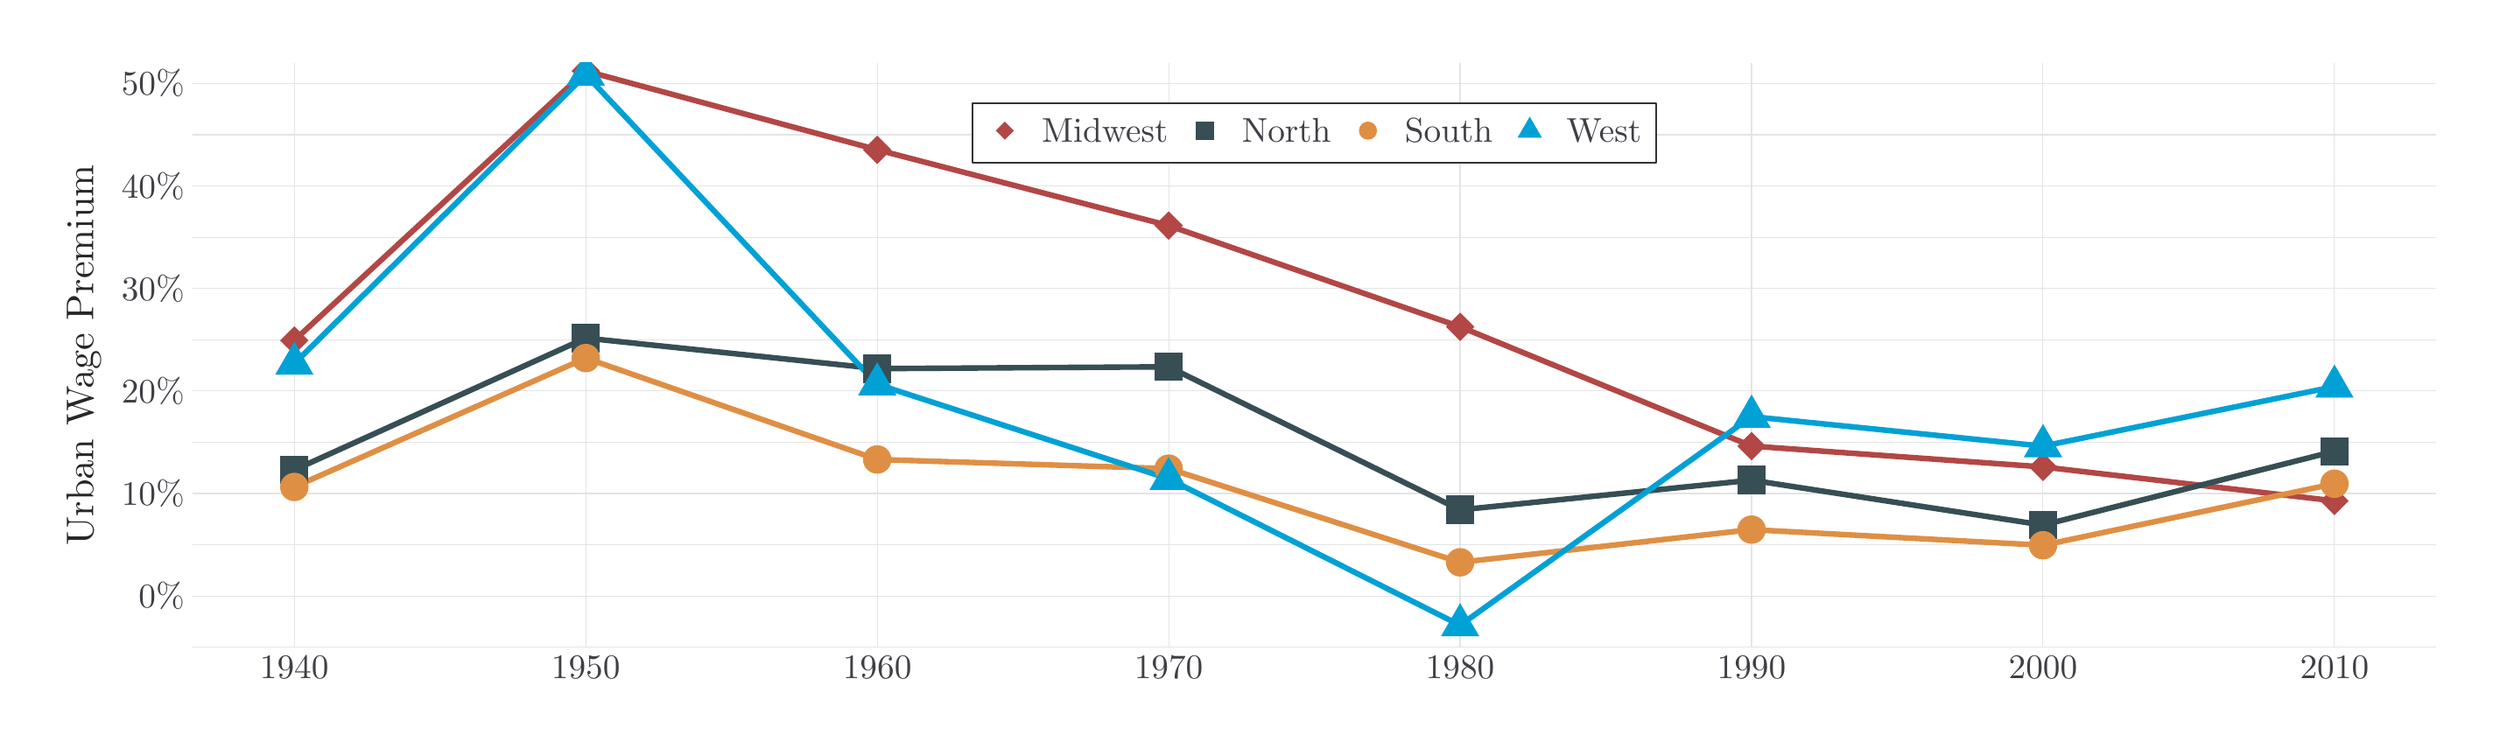
\begin{tikzpicture}[x=1pt,y=1pt]
\definecolor{fillColor}{RGB}{255,255,255}
\path[use as bounding box,fill=fillColor] (0,0) rectangle (1011.78,289.08);
\begin{scope}
\path[clip] (  0.00,  0.00) rectangle (1011.78,289.08);
\definecolor{drawColor}{RGB}{255,255,255}

\path[draw=drawColor,line width= 0.8pt,line join=round,line cap=round,fill=fillColor] (  0.00,  0.00) rectangle (1011.78,289.08);
\end{scope}
\begin{scope}
\path[clip] ( 69.39, 31.76) rectangle (995.78,273.08);
\definecolor{drawColor}{RGB}{255,255,255}
\definecolor{fillColor}{RGB}{255,255,255}

\path[draw=drawColor,line width= 0.8pt,line join=round,line cap=round,fill=fillColor] ( 69.39, 31.76) rectangle (995.78,273.08);
\definecolor{drawColor}{RGB}{228,228,231}

\path[draw=drawColor,line width= 0.4pt,line join=round] ( 69.39, 31.76) --
	(995.78, 31.76);

\path[draw=drawColor,line width= 0.4pt,line join=round] ( 69.39, 74.10) --
	(995.78, 74.10);

\path[draw=drawColor,line width= 0.4pt,line join=round] ( 69.39,116.43) --
	(995.78,116.43);

\path[draw=drawColor,line width= 0.4pt,line join=round] ( 69.39,158.77) --
	(995.78,158.77);

\path[draw=drawColor,line width= 0.4pt,line join=round] ( 69.39,201.11) --
	(995.78,201.11);

\path[draw=drawColor,line width= 0.4pt,line join=round] ( 69.39,243.44) --
	(995.78,243.44);

\path[draw=drawColor,line width= 0.4pt,line join=round] ( 69.39, 52.93) --
	(995.78, 52.93);

\path[draw=drawColor,line width= 0.4pt,line join=round] ( 69.39, 95.26) --
	(995.78, 95.26);

\path[draw=drawColor,line width= 0.4pt,line join=round] ( 69.39,137.60) --
	(995.78,137.60);

\path[draw=drawColor,line width= 0.4pt,line join=round] ( 69.39,179.94) --
	(995.78,179.94);

\path[draw=drawColor,line width= 0.4pt,line join=round] ( 69.39,222.28) --
	(995.78,222.28);

\path[draw=drawColor,line width= 0.4pt,line join=round] ( 69.39,264.61) --
	(995.78,264.61);

\path[draw=drawColor,line width= 0.4pt,line join=round] (111.50, 31.76) --
	(111.50,273.08);

\path[draw=drawColor,line width= 0.4pt,line join=round] (231.81, 31.76) --
	(231.81,273.08);

\path[draw=drawColor,line width= 0.4pt,line join=round] (352.12, 31.76) --
	(352.12,273.08);

\path[draw=drawColor,line width= 0.4pt,line join=round] (472.43, 31.76) --
	(472.43,273.08);

\path[draw=drawColor,line width= 0.4pt,line join=round] (592.74, 31.76) --
	(592.74,273.08);

\path[draw=drawColor,line width= 0.4pt,line join=round] (713.05, 31.76) --
	(713.05,273.08);

\path[draw=drawColor,line width= 0.4pt,line join=round] (833.36, 31.76) --
	(833.36,273.08);

\path[draw=drawColor,line width= 0.4pt,line join=round] (953.67, 31.76) --
	(953.67,273.08);
\definecolor{drawColor}{RGB}{178,71,69}

\path[draw=drawColor,line width= 2.3pt,line join=round] (111.50,158.51) --
	(231.81,269.76) --
	(352.12,237.23) --
	(472.43,205.91) --
	(592.74,164.12) --
	(713.05,114.86) --
	(833.36,106.25) --
	(953.67, 92.23);
\definecolor{drawColor}{RGB}{55,78,85}

\path[draw=drawColor,line width= 2.3pt,line join=round] (111.50,105.01) --
	(231.81,159.45) --
	(352.12,146.85) --
	(472.43,147.59) --
	(592.74, 88.52) --
	(713.05,100.78) --
	(833.36, 82.24) --
	(953.67,112.70);
\definecolor{drawColor}{RGB}{223,143,68}

\path[draw=drawColor,line width= 2.3pt,line join=round] (111.50, 97.98) --
	(231.81,151.20) --
	(352.12,109.32) --
	(472.43,105.55) --
	(592.74, 66.86) --
	(713.05, 80.36) --
	(833.36, 73.91) --
	(953.67, 99.31);
\definecolor{drawColor}{RGB}{0,161,213}

\path[draw=drawColor,line width= 2.3pt,line join=round] (111.50,148.90) --
	(231.81,268.23) --
	(352.12,140.38) --
	(472.43,101.35) --
	(592.74, 40.87) --
	(713.05,127.03) --
	(833.36,114.84) --
	(953.67,139.41);
\definecolor{fillColor}{RGB}{178,71,69}

\path[fill=fillColor] (105.63,158.51) --
	(111.50,164.38) --
	(117.37,158.51) --
	(111.50,152.64) --
	cycle;
\definecolor{fillColor}{RGB}{55,78,85}

\path[fill=fillColor] (105.63, 99.14) --
	(117.37, 99.14) --
	(117.37,110.88) --
	(105.63,110.88) --
	cycle;
\definecolor{fillColor}{RGB}{223,143,68}

\path[fill=fillColor] (111.50, 97.98) circle (  5.87);
\definecolor{fillColor}{RGB}{0,161,213}

\path[fill=fillColor] (111.50,158.03) --
	(119.41,144.33) --
	(103.59,144.33) --
	cycle;
\definecolor{fillColor}{RGB}{178,71,69}

\path[fill=fillColor] (225.94,269.76) --
	(231.81,275.63) --
	(237.68,269.76) --
	(231.81,263.89) --
	cycle;
\definecolor{fillColor}{RGB}{55,78,85}

\path[fill=fillColor] (225.94,153.57) --
	(237.68,153.57) --
	(237.68,165.32) --
	(225.94,165.32) --
	cycle;
\definecolor{fillColor}{RGB}{223,143,68}

\path[fill=fillColor] (231.81,151.20) circle (  5.87);
\definecolor{fillColor}{RGB}{0,161,213}

\path[fill=fillColor] (231.81,277.36) --
	(239.72,263.67) --
	(223.90,263.67) --
	cycle;
\definecolor{fillColor}{RGB}{178,71,69}

\path[fill=fillColor] (346.25,237.23) --
	(352.12,243.10) --
	(357.99,237.23) --
	(352.12,231.36) --
	cycle;
\definecolor{fillColor}{RGB}{55,78,85}

\path[fill=fillColor] (346.25,140.98) --
	(357.99,140.98) --
	(357.99,152.72) --
	(346.25,152.72) --
	cycle;
\definecolor{fillColor}{RGB}{223,143,68}

\path[fill=fillColor] (352.12,109.32) circle (  5.87);
\definecolor{fillColor}{RGB}{0,161,213}

\path[fill=fillColor] (352.12,149.51) --
	(360.03,135.81) --
	(344.21,135.81) --
	cycle;
\definecolor{fillColor}{RGB}{178,71,69}

\path[fill=fillColor] (466.56,205.91) --
	(472.43,211.78) --
	(478.30,205.91) --
	(472.43,200.03) --
	cycle;
\definecolor{fillColor}{RGB}{55,78,85}

\path[fill=fillColor] (466.56,141.72) --
	(478.30,141.72) --
	(478.30,153.46) --
	(466.56,153.46) --
	cycle;
\definecolor{fillColor}{RGB}{223,143,68}

\path[fill=fillColor] (472.43,105.55) circle (  5.87);
\definecolor{fillColor}{RGB}{0,161,213}

\path[fill=fillColor] (472.43,110.48) --
	(480.34, 96.78) --
	(464.52, 96.78) --
	cycle;
\definecolor{fillColor}{RGB}{178,71,69}

\path[fill=fillColor] (586.87,164.12) --
	(592.74,169.99) --
	(598.61,164.12) --
	(592.74,158.24) --
	cycle;
\definecolor{fillColor}{RGB}{55,78,85}

\path[fill=fillColor] (586.87, 82.64) --
	(598.61, 82.64) --
	(598.61, 94.39) --
	(586.87, 94.39) --
	cycle;
\definecolor{fillColor}{RGB}{223,143,68}

\path[fill=fillColor] (592.74, 66.86) circle (  5.87);
\definecolor{fillColor}{RGB}{0,161,213}

\path[fill=fillColor] (592.74, 50.01) --
	(600.65, 36.31) --
	(584.83, 36.31) --
	cycle;
\definecolor{fillColor}{RGB}{178,71,69}

\path[fill=fillColor] (707.18,114.86) --
	(713.05,120.74) --
	(718.92,114.86) --
	(713.05,108.99) --
	cycle;
\definecolor{fillColor}{RGB}{55,78,85}

\path[fill=fillColor] (707.18, 94.91) --
	(718.92, 94.91) --
	(718.92,106.66) --
	(707.18,106.66) --
	cycle;
\definecolor{fillColor}{RGB}{223,143,68}

\path[fill=fillColor] (713.05, 80.36) circle (  5.87);
\definecolor{fillColor}{RGB}{0,161,213}

\path[fill=fillColor] (713.05,136.16) --
	(720.96,122.46) --
	(705.14,122.46) --
	cycle;
\definecolor{fillColor}{RGB}{178,71,69}

\path[fill=fillColor] (827.49,106.25) --
	(833.36,112.12) --
	(839.23,106.25) --
	(833.36,100.38) --
	cycle;
\definecolor{fillColor}{RGB}{55,78,85}

\path[fill=fillColor] (827.49, 76.36) --
	(839.23, 76.36) --
	(839.23, 88.11) --
	(827.49, 88.11) --
	cycle;
\definecolor{fillColor}{RGB}{223,143,68}

\path[fill=fillColor] (833.36, 73.91) circle (  5.87);
\definecolor{fillColor}{RGB}{0,161,213}

\path[fill=fillColor] (833.36,123.97) --
	(841.27,110.27) --
	(825.45,110.27) --
	cycle;
\definecolor{fillColor}{RGB}{178,71,69}

\path[fill=fillColor] (947.80, 92.23) --
	(953.67, 98.10) --
	(959.54, 92.23) --
	(953.67, 86.36) --
	cycle;
\definecolor{fillColor}{RGB}{55,78,85}

\path[fill=fillColor] (947.80,106.83) --
	(959.54,106.83) --
	(959.54,118.58) --
	(947.80,118.58) --
	cycle;
\definecolor{fillColor}{RGB}{223,143,68}

\path[fill=fillColor] (953.67, 99.31) circle (  5.87);
\definecolor{fillColor}{RGB}{0,161,213}

\path[fill=fillColor] (953.67,148.55) --
	(961.58,134.85) --
	(945.76,134.85) --
	cycle;
\end{scope}
\begin{scope}
\path[clip] (  0.00,  0.00) rectangle (1011.78,289.08);
\definecolor{drawColor}{RGB}{63,63,70}

\node[text=drawColor,anchor=base east,inner sep=0pt, outer sep=0pt, scale=  1.42] at ( 66.19, 48.03) {0\%};

\node[text=drawColor,anchor=base east,inner sep=0pt, outer sep=0pt, scale=  1.42] at ( 66.19, 90.37) {10\%};

\node[text=drawColor,anchor=base east,inner sep=0pt, outer sep=0pt, scale=  1.42] at ( 66.19,132.70) {20\%};

\node[text=drawColor,anchor=base east,inner sep=0pt, outer sep=0pt, scale=  1.42] at ( 66.19,175.04) {30\%};

\node[text=drawColor,anchor=base east,inner sep=0pt, outer sep=0pt, scale=  1.42] at ( 66.19,217.38) {40\%};

\node[text=drawColor,anchor=base east,inner sep=0pt, outer sep=0pt, scale=  1.42] at ( 66.19,259.72) {50\%};
\end{scope}
\begin{scope}
\path[clip] (  0.00,  0.00) rectangle (1011.78,289.08);
\definecolor{drawColor}{RGB}{63,63,70}

\node[text=drawColor,anchor=base,inner sep=0pt, outer sep=0pt, scale=  1.42] at (111.50, 18.76) {1940};

\node[text=drawColor,anchor=base,inner sep=0pt, outer sep=0pt, scale=  1.42] at (231.81, 18.76) {1950};

\node[text=drawColor,anchor=base,inner sep=0pt, outer sep=0pt, scale=  1.42] at (352.12, 18.76) {1960};

\node[text=drawColor,anchor=base,inner sep=0pt, outer sep=0pt, scale=  1.42] at (472.43, 18.76) {1970};

\node[text=drawColor,anchor=base,inner sep=0pt, outer sep=0pt, scale=  1.42] at (592.74, 18.76) {1980};

\node[text=drawColor,anchor=base,inner sep=0pt, outer sep=0pt, scale=  1.42] at (713.05, 18.76) {1990};

\node[text=drawColor,anchor=base,inner sep=0pt, outer sep=0pt, scale=  1.42] at (833.36, 18.76) {2000};

\node[text=drawColor,anchor=base,inner sep=0pt, outer sep=0pt, scale=  1.42] at (953.67, 18.76) {2010};
\end{scope}
\begin{scope}
\path[clip] (  0.00,  0.00) rectangle (1011.78,289.08);
\definecolor{drawColor}{RGB}{39,39,42}

\node[text=drawColor,rotate= 90.00,anchor=base,inner sep=0pt, outer sep=0pt, scale=  1.60] at ( 28.57,152.42) {Urban Wage Premium};
\end{scope}
\begin{scope}
\path[clip] (  0.00,  0.00) rectangle (1011.78,289.08);
\definecolor{drawColor}{gray}{0.20}
\definecolor{fillColor}{RGB}{255,255,255}

\path[draw=drawColor,line width= 0.8pt,line join=round,line cap=round,fill=fillColor] (391.59,231.89) rectangle (673.59,256.35);
\end{scope}
\begin{scope}
\path[clip] (  0.00,  0.00) rectangle (1011.78,289.08);
\definecolor{drawColor}{RGB}{255,255,255}
\definecolor{fillColor}{RGB}{255,255,255}

\path[draw=drawColor,line width= 0.8pt,line join=round,line cap=round,fill=fillColor] (397.59,237.89) rectangle (412.04,252.35);

\path[] (399.03,245.12) -- (410.60,245.12);
\definecolor{fillColor}{RGB}{178,71,69}

\path[fill=fillColor] (401.08,245.12) --
	(404.81,248.85) --
	(408.54,245.12) --
	(404.81,241.39) --
	cycle;
\end{scope}
\begin{scope}
\path[clip] (  0.00,  0.00) rectangle (1011.78,289.08);
\definecolor{drawColor}{RGB}{255,255,255}
\definecolor{fillColor}{RGB}{255,255,255}

\path[draw=drawColor,line width= 0.8pt,line join=round,line cap=round,fill=fillColor] (480.25,237.89) rectangle (494.70,252.35);

\path[] (481.69,245.12) -- (493.26,245.12);
\definecolor{fillColor}{RGB}{55,78,85}

\path[fill=fillColor] (483.74,241.39) --
	(491.20,241.39) --
	(491.20,248.85) --
	(483.74,248.85) --
	cycle;
\end{scope}
\begin{scope}
\path[clip] (  0.00,  0.00) rectangle (1011.78,289.08);
\definecolor{drawColor}{RGB}{255,255,255}
\definecolor{fillColor}{RGB}{255,255,255}

\path[draw=drawColor,line width= 0.8pt,line join=round,line cap=round,fill=fillColor] (547.47,237.89) rectangle (561.92,252.35);

\path[] (548.91,245.12) -- (560.47,245.12);
\definecolor{fillColor}{RGB}{223,143,68}

\path[fill=fillColor] (554.69,245.12) circle (  3.73);
\end{scope}
\begin{scope}
\path[clip] (  0.00,  0.00) rectangle (1011.78,289.08);
\definecolor{drawColor}{RGB}{255,255,255}
\definecolor{fillColor}{RGB}{255,255,255}

\path[draw=drawColor,line width= 0.8pt,line join=round,line cap=round,fill=fillColor] (614.25,237.89) rectangle (628.71,252.35);

\path[] (615.70,245.12) -- (627.26,245.12);
\definecolor{fillColor}{RGB}{0,161,213}

\path[fill=fillColor] (621.48,250.92) --
	(626.50,242.22) --
	(616.45,242.22) --
	cycle;
\end{scope}
\begin{scope}
\path[clip] (  0.00,  0.00) rectangle (1011.78,289.08);
\definecolor{drawColor}{RGB}{63,63,70}

\node[text=drawColor,anchor=base west,inner sep=0pt, outer sep=0pt, scale=  1.42] at (420.04,240.22) {Midwest};
\end{scope}
\begin{scope}
\path[clip] (  0.00,  0.00) rectangle (1011.78,289.08);
\definecolor{drawColor}{RGB}{63,63,70}

\node[text=drawColor,anchor=base west,inner sep=0pt, outer sep=0pt, scale=  1.42] at (502.70,240.22) {North};
\end{scope}
\begin{scope}
\path[clip] (  0.00,  0.00) rectangle (1011.78,289.08);
\definecolor{drawColor}{RGB}{63,63,70}

\node[text=drawColor,anchor=base west,inner sep=0pt, outer sep=0pt, scale=  1.42] at (569.92,240.22) {South};
\end{scope}
\begin{scope}
\path[clip] (  0.00,  0.00) rectangle (1011.78,289.08);
\definecolor{drawColor}{RGB}{63,63,70}

\node[text=drawColor,anchor=base west,inner sep=0pt, outer sep=0pt, scale=  1.42] at (636.71,240.22) {West};
\end{scope}
\end{tikzpicture}
